
\section{Optimierung des DSP}
Nach dem in dem vorherigen Kapitel die Optimierung des Musikklassifikators aufm dem ARM Cortex-A8 beschrieben wurde, behandelt dieses Kapitel die Optimierung der Extraktionsphase auf dem C674x DSP von Texas Instruments.\\
Als erstes muss der C++-Referenzcode in C-Code �bersetzt werden, da der C674x nur diesen ausf�hren kann. Anschlie�end werden durch eine Laufzeitmessung die Laufzeitantiele der einzelnen Feature-Berechnungen ermittelt (siehe \textbf{Abbildung \ref{fig:startdsp}}).
%
\begin{figure}[h]
	\centering
		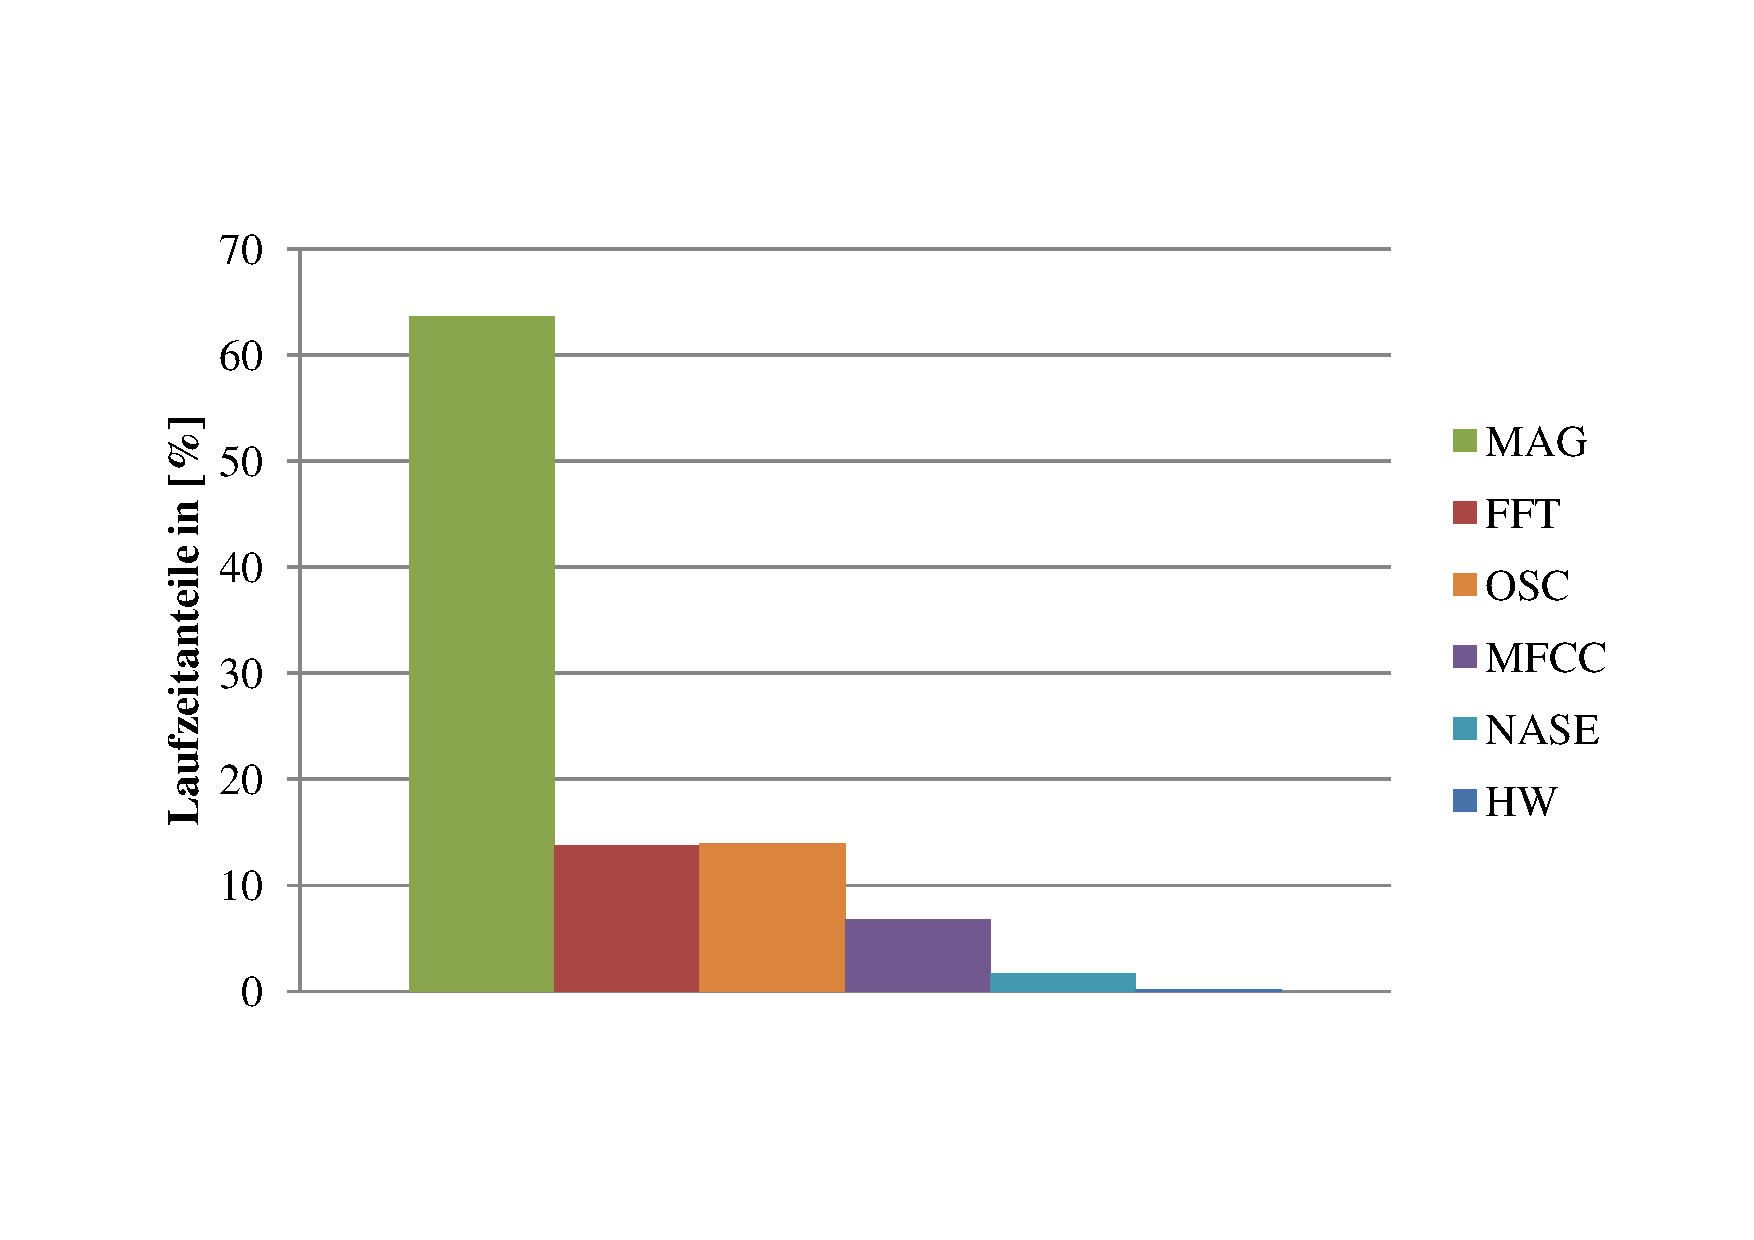
\includegraphics[width=1\textwidth]{../Pictures/startdsp.pdf}
	\caption{Laufzeitanteile der einzelnen Features}
	\label{fig:startdsp}
\end{figure} 
%
Wie man der Abbildung entnehmen kann f�llt der gr��te Anteil mit �ber 60\% der Magnitude of Spectrum zu, aber auch FFT und Octave Spectral Contrast mit je 14\% sind nicht zu vernachl�ssigen.\\
Ein Detailprofiling der Magnitude of Spectrum ergibt, dass 

\subsection{Optimierung der Rechenfunktionen mit MATHLIB}\label{sec:mathlib}
Da wie bereits erw�hnt, die Rechenfunktionen bei zum Beispiel der Magnitude of Spectrum als Bottlenecks identifiziert wurden und wie in \textbf{Kapitel \ref{subsubsec:optbib}} erw�hnt eine Bibliothek (MATHLIB) existiert, in der genau diese Rechenoperationen optimiert wurden, werden alle problematischen Funktionen durch ihre optimierten Varianten ersetzt. Wie ebenfalls in dem Kapitel erw�hnt, existieren f�r alle in MATHLIB implementierten Operationen auch Varianten, die auf Vektoren von Eingangswerten arbeiten k�nnen. Daher wird als erstes versucht, soweit es m�glich ist, Operationen wie zum Beispiel Divisionen, Wurzelberechnungen oder Logarithmusfunktionen durch diese Vektoroperationen zu ersetzten. Sollte eine Ersetzung durch Vektoroperationen nicht m�glich sein, werden Einzelaufrufe durch die optimierten Varianten der MATHLIB ersetzt.\\
Diese Ersetzung wird Beispielhaft f�r Magnitude of Spectrum in \textbf{Listing \ref{code:aosc}} und \textbf{Listing \ref{code:aosm}} gezeigt.
\newpage
\begin{lstlisting}[caption=Referenzcode von Magnitude of Spectrum, label=code:aosc]
	A[k] = sqrt(X[k] * X[k] + Y[k] * Y[k]) / G;
\end{lstlisting}

\begin{lstlisting}[caption=Magnitude of Spectrum mit MATHLIB, label=code:aosm]
	for (k = 0; k < G; ++k) {
		tmp1 = X[k] * X[k];
		tmp2 = Y[k] * Y[k];
		A[k] = (tmp1 + tmp2); //(X[k] * X[k] + Y[k] * Y[k]);
	}
	
	sqrtsp_v(A, A, G);

	divsp_v(A, pG, A, G);
\end{lstlisting}

Die Akkumulation innerhalb der Wurzelberechnung wurde zus�tzlich f�r eine bessere Ausf�hrung durch SPLOOP getrennt.\\
Eine Optimierung mit MATHLIB wurde bei folgenden Algorithmen durchgef�hrt:

\begin{itemize}
\item Magnitude of Spectrum
\item MFCC
\item Low Energy
\item Normalized Audio Spectrum Envelope
\item Octave Spectral Contrast
\item Root Mean Square
\item Spectral Centroid
\item Spectral Crest Factor
\item Spectral Flux
\item Sub-band Energy Ratio
\end{itemize}

\subsection{Optimierung der FFT mit DSPLIB}\label{sec:dsplib}

\subsection{Optimierung f�r den Compiler}\label{sec:compiler} 